
% Copyright 2004 by Till Tantau <tantau@users.sourceforge.net>.
%
% In principle, this file can be redistributed and/or modified under
% the terms of the GNU Public License, version 2.
%
% However, this file is supposed to be a template to be modified
% for your own needs. For this reason, if you use this file as a
% template and not specifically distribute it as part of a another
% package/program, I grant the extra permission to freely copy and
% modify this file as you see fit and even to delete this copyright
% notice. 

\documentclass[xcolor={dvipsnames}]{beamer}

\usetheme{Madrid}
\usepackage[lithuanian]{babel}
\usepackage[utf8x]{inputenc}
\usepackage{lmodern}
\usepackage[L7x]{fontenc}
%\usepackage{times}
%\usepackage{verbatim}
\usepackage{cancel}
\usepackage{graphicx}
\usepackage{fancyvrb}
\usepackage{bm}
\usepackage{amsfonts, amsmath, amssymb}
\usepackage{float}
\usepackage{hyperref}
\usepackage{caption}
\usepackage{subfig}
\usepackage{comment}
\usepackage{multicol}
\usepackage{hyperref}
\usepackage{tabularx}
\usepackage{diagbox} %diag tables

\title{Kaip matematikos mokymo teoriją įgyvendinti tikrovėje?}
\author{Simonas Mamaitis}
\date{2021 03 03}


% Let's get started
\begin{document}

\begin{frame}
  \titlepage
\end{frame}

%\begin{frame}{Turinys} \tableofcontents \end{frame}

\begin{frame}[fragile]{Pagrindinis retorinis klausimas}
\begin{itemize}
\item<1-> Tarkime labai gerai išstudijavome daugybės matematinių uždavinių sandarą. Kaip tai gali panaudota pakelti mokymosi proceso kokybę pamokose?
	\begin{itemize}
		\item <2-> Disertacijos - padės rengiant mokytojus?
		\item <3-> Matematikos populiarinimas - ar verta sprendimus kelti į tą žurnalą?
		\item <4-> Kiti moksleiviams ir mokytojams padedantys produktai - kuo tai bus naudingiau už tai, kas jau sukurta? 
		\item <5-> Simono vienas iš atsakymų: \textbf{uždavinių duomenys} gali padėti atsakyti, koks turėtų būti matematikos mokymo turinys ir jo išsidėstymas.
		\item <6-> Jei prie šių duomenų prijungtume \textbf{mokinių pasiekimų duomenis}, turėtume \textbf{duomenų bazę}, kuriai tereikia geros valdymo sistemos.
		\item <7-> Išvada: \textbf{duomenų analizė} - reikšmingas metodas, kurį galima taikyti matematikos turinio kūrime.
	\end{itemize}
\end{itemize}
\end{frame}

\begin{frame}[fragile]{Duomenų modelis 1}
\begin{itemize}
\item<1-> Kiekvienas uždavinys yra konvertuojamas į atskirus žingsnius, kurių kiekviename išlaikoma čia pateikiama duomenų struktūra.
\item<2-> Imame tam tikrą sprendimo žingsnį ir bandome rasti griežtą paaiškinimą, kodėl jis galioja.
\item<3-> Stebime, ar taisyklės paaiškinimas veiksmingas pamokoje. Jei ne, galbūt norint jį perprasti moksleiviams reikia kitų taisyklių, įgūdžių ar paaiškinimų.
      \begin{itemize}
	\item<4-> $\boxed{\boxed{\text{Teiginys}} \stackrel{\boxed{\text{Sprendimo žingsnis}}}{\Rightarrow} \boxed{\text{Kita teiginio forma}}}$
	\item<5-> $\boxed{\boxed{\text{Teiginys}} \stackrel{\begin{array}{c}\boxed{\text{Taisyklė}}\\ \Downarrow\end{array}}{\Longrightarrow} \boxed{\text{Kita teiginio forma}}}$
	\item<6-> $\boxed{\boxed{\text{Teiginys}} \stackrel{\begin{array}{l}\boxed{\text{Taisyklė}}\\ \qquad\Downarrow\Leftarrow\boxed{\text{Kitos žinios}}\end{array}}{\xrightarrow{\hspace*{3cm}}} \boxed{\text{Kita teiginio forma}}}$
      \end{itemize}
\end{itemize}
\end{frame}

\begin{frame}[fragile]{Duomenų modelio 1 praktinė nauda}
\begin{itemize}
\item<1->  Šio modelio tikslas yra nustatyti galimą mokymo turinio formavimą (TF) ir išdėstymą (TI).
\item<2->  Pavyzdžiui mokykloje mokoma spręsti lygtis perkeliant vienanarius į kitą lygybės pusę. Galima pasiūlyti tokį TF būdą:
\begin{itemize}
\item Vienas iš lygties \textbf{sprendimo žingsnių} - skaičiaus perkėlimas į kitą lygties pusę.
\item Perkėlimas įmanomas pagal \textbf{taisyklę}, kad galima pridėti po tą patį prie abiejų pusių
\item Norint suprasti, kodėl galima pridėti po tą patį, reikia \textbf{kitų žinių}. Gali padėti lygties siejimas su svarstyklėmis.
\end{itemize}
\end{itemize}
\end{frame}


\begin{frame}[fragile]{Duomenų modelio 1 realizavimo pavyzdys 1}
Pitagoro teoremos įrodymas

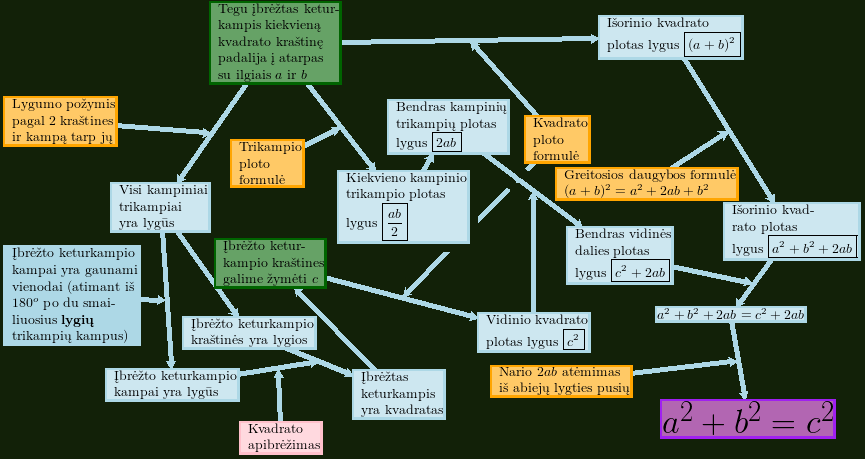
\includegraphics[width=\textwidth]{pyth1.png}
\end{frame}

\begin{frame}[fragile]{Duomenų modelio 1 realizavimo pavyzdys 1}
Pitagoro teoremos įrodymas

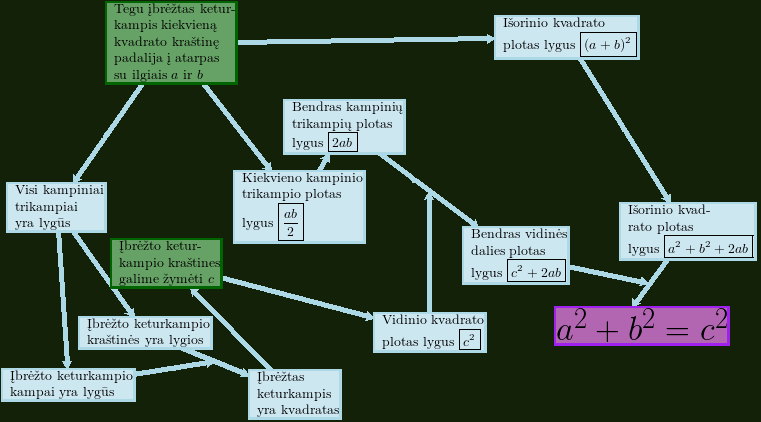
\includegraphics[width=\textwidth]{pyth2.png}
\end{frame}

\begin{frame}[fragile]{Duomenų modelio 1 realizavimo pavyzdys 1}
Pitagoro teoremos įrodymas

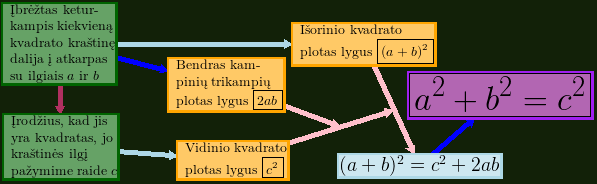
\includegraphics[width=\textwidth]{pyth3.png}
\end{frame}

\begin{frame}[fragile]{Duomenų modelio 1 realizavimo pavyzdys 1}
\begin{itemize}
\item<1-> Pitagoro teoremos įrodymas

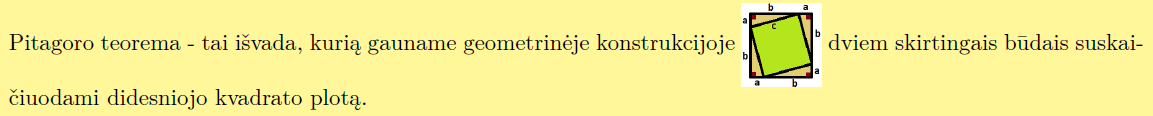
\includegraphics[width=0.9\textwidth]{pyth4.png}

\item<2-> Apie šį įrodymą plačiau pasakojama ieškant atsakymų, \href{https://github.com/loijord/General/blob/master/READING/proofs\_and\_memory/kaip\_atkurti\_matematika\_atmintyje.pdf}{kaip matematinės žinios tampa atkuriamomis atmintyje}
\end{itemize}
\end{frame}

\begin{frame}[fragile]{Duomenų modelio 1 realizavimo pavyzdys 2}
\begin{itemize}
\item<1-> Lygybės $(a^n)^m = a^{nm}$ įrodymas.

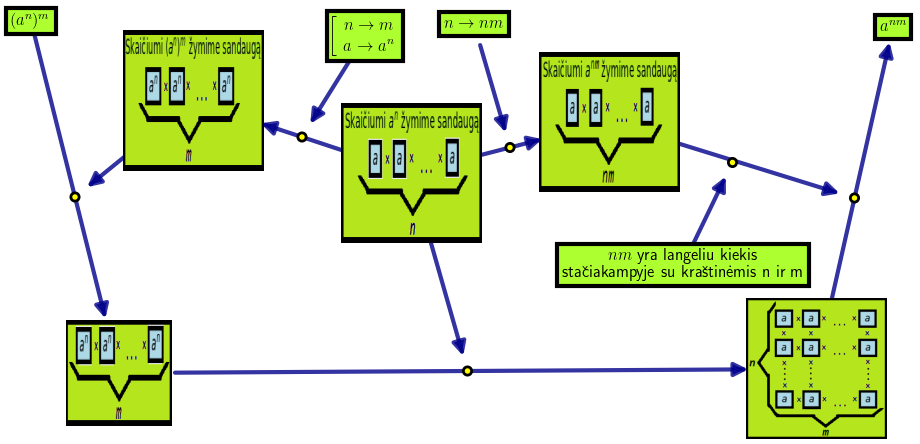
\includegraphics[width=0.9\textwidth]{neuro_output.png}

\item<2-> Šis įrodymas, kaip ir Pitagoro teoremos įrodymas, leidžia pamatyti, kas buvo taikyta ir kiek dažnai. Įdomu, kad prireikė dalies, kuri reikalinga taip pat ir ploto sampratoje.
\end{itemize}
\end{frame}

\begin{frame}[fragile]{Duomenų modelio 1 praktinė nauda}
\begin{itemize}
\item<1-> Rezultatas: galima kelti ir tikrinti prielaidas apie TF ir TI. Čia pateiksime jų pavyzdžius:
 \begin{itemize}
	\item Prielaida 1 apie TI. Lygtis spręsti reiktų mokyti vyresnėse klasėse $^{???}$
	\item Prielaida 2 apie TI. Moksleivius reikia labiau supažindinti su realiųjų skaičių savybėmis, kurios įeina į lygčių sprendimo taisykles.
	\item Prielaida 3 apie TI. Lygtims mokytis skiriama per mažai/per daug laiko.
	\item Prielaida 4 apie TF. Mokymo programoje aiškinant lygčių sprendimą nėra įtraukta \textbf{taisyklė} arba taisyklės aiškinime nesiremiama tam reikiamomis \textbf{kitomis žiniomis}
	\item Prielaida 5 apie TF. \textbf{Taisyklė} įtraukta, tačiau ankstesnėse pamokose prastai išplėtota, todėl būtina pasirūpinti jos formavimu ankstesniame turinyje.
	\item Prielaida 6 apie TF/TI. Pagal \textbf{taisyklės} taikymo dažnumą įvairiose temose galima spręsti, kurią dalį pamokų skirsime kalbėti apie tą taisyklę.
\end{itemize}
\end{itemize}
\end{frame}

\begin{frame}[fragile]{Duomenų modelis 1: kokios galimybės jį realizuoti?}
\begin{itemize}
\item<1-> Kai kurie samprotavimo elementai sunkiai aprašomi. Pvz. \textit{Modus Ponens} principas arba \textit{įrodymas prieštaros metodu}.
\item<2-> Uždaviniai ir taisyklės gali turėti po kelias schemas.
\item<3-> Nagrinėjant uždavinius atsiranda labai daug duomenų, tam reikia daug rankų.
\item<4-> Ši duomenų struktūra sudėtinga, reikalaujanti daug nusimanyti apie duomenų bazių valdymą.
\item<5-> Retorinis klausimas - ar gali būti pasiektas \textbf{tikslas}?
\item<6-> $^{???}$ Modelyje naudojamos tik žinios apie uždavinius, tačiau neatsižvelgiama į mokinių pasiekimus. Natūralu, kad reikia šį modelį praplėsti.
\end{itemize}
\end{frame}

\begin{frame}[fragile]{Kaip įtraukti į duomenų modelį 1 moksleivių pasiekimus?}
Citata iš \textit{Liping Ma} knygos \textit{Knowing and teaching elementary mathematics} apie Kinijoje naudojamus Teacher's manuals. The main body of the manual is a section-by-section discussion of each topic and subtopic of the textbook. The discussion of each topic focuses on these questions:
\begin{itemize}
\item<1-> What is the concept connected with the topic?
\item<2-> What are the difficult points of teaching the concept?
\item<3-> What are the important points of teaching the concept?
\item<4-> What are the errors and confusions that students tend to have when learning this topic?
\end{itemize}
\end{frame}

\begin{frame}[fragile]{Nuveiktų darbų pavyzdžiai}
Duomenų modelis 1 tikslo nepasiekė: nebuvo sukurta duomenų bazė, kuria remiantis būtų galima kelti ir tikrinti prielaidas apie TF ir TI. Tačiau jo idėjos įkvėpė sukurti teorinę medžiagą, atitinkamus uždavinius ir užsiėmimų aprašymus. 
\begin{itemize}
\item<1-> Pavyzdys 1: \href{https://github.com/loijord/matematikos\_pamokos/blob/master/programa/Mantas/Projektas2/dauginimas.pdf} tema apie dauginimus.
\item<2-> Pavyzdys 2: \href{https://github.com/loijord/General/blob/master/READING/project\_topics/fraktalai/fraktalai.pdf}{dialogas su mokiniu apie fraktalus}
\item<3-> Pavyzdys 3: įvairi mokomoji medžiaga, laukianti dienos šviesos (bus šio seminaro prieduose)
\item<4-> Pavyzdys 4: pagal valstybinio egzamino uždavinius sudaryta \href{https://github.com/loijord/egzanalysis/tree/master/READING}{mokomoji medžiaga}, skirta ruoštis egzaminui.
\item<5-> Pavyzdys 5: daugiau nei 30 tikrovėje vykusių užsiėmimų aprašymų, \href{https://github.com/loijord/matematikos\_pamokos/tree/master/programa}{įkeltų į internetą} (copyrights?)
\item<6-> Pavyzdys 6: gamification kaip matematikos mokymo priemonė.
\end{itemize}
\end{frame}

\begin{frame}[fragile]{Duomenų modelis 2}
\begin{itemize}
\item<1-> Kai Simonas įgyjo šiek tiek daugiau žinių apie duomenų bazių (DB) valdymą, atsirado veiksmingas būdas
\begin{itemize}
\item<2-> rinkti informaciją apie konkretaus moksleivio pasiekimus
\item<3-> rinkti informaciją apie konkretaus testo sandarą
\item<4-> naudojant užklausas paspartinti pamokų darbą.
\end{itemize}
\item<5-> Duomenų sistemą sudaro dvi DB: tam tikro testo uždavinių DB ir moksleivio pasiekimų DB.
\item<6-> Nepaisant didelių laiko nuostolių įvedinėjant uždavinius ir pasiekimus, tai veikia!
\end{itemize}
\end{frame}

\begin{frame}[fragile]{Duomenų modelis 2: uždavinių DB}
\begin{itemize}
\item<1-> Uždavinių DB gali sudaryti tam tikrų metų egzamino, stojamojo į gimnaziją arba Simono sudaryti uždaviniai.
\item<2-> Egzaminui arba stojamajam turi būti aiškus testuojamų gebėjimų sąrašas
\item<3-> Kiekvienas uždavinys aprašomas tokiais duomenimis:

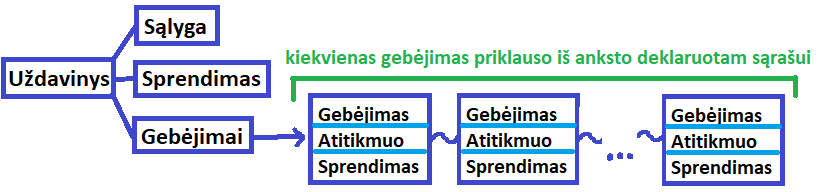
\includegraphics[width=0.9\textwidth]{problem_db.png}

\item<4-> \href{https://github.com/loijord/matematikos\_pamokos/blob/master/programa/database/generavimas/licejus\_2017.ipynb}{Pavyzdys, kaip vyksta uždavinių įvedinėjimas}
\end{itemize}
\end{frame}


\begin{frame}[fragile]{Duomenų modelis 2: pasiekimų DB}
\begin{itemize}
\item<1-> Pasiekimų DB sudaro uždaviniai, jų dalys ir atsakymai, ar moksleiviui pavyko išspręsti tuos uždavinius ar jų dalis.

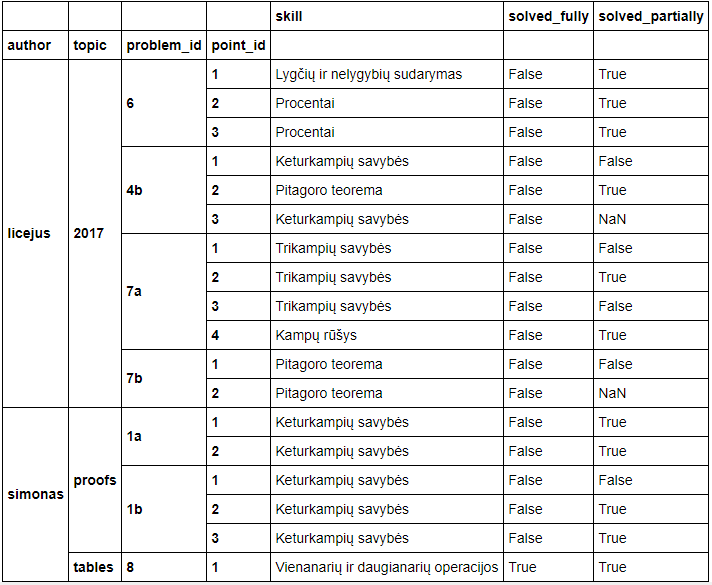
\includegraphics[width=0.7\textwidth]{skills_db.png}
\end{itemize}
\end{frame}

\begin{frame}[fragile]{Duomenų modelis 2: už ir prieš}
\begin{itemize}
\item<1->  Detali uždavinių turinio analizė iškeičiama į moksleivių pasiekimų analizę. Netinkamą tam tikros temos TF arba TI atskleidžia ne uždavinio sandara, o prasti moksleivių rezultatai.
\item<2->  Stebima tendencija: gebėjimų atlikti atskiras dalis tarsi yra, bet jie nekombinuojami tarpusavyje ir uždavinių moksleiviams iki galo išspręsti nepavyksta.
\item<3->  Uždavinių sprendimo žingsniai - vienodo svorio. Ruošiantis stojamajam ar egzaminui stengiamasi imituoti tame teste naudojamą vertinimą.
\item<4->  Kada verta vieną sprendimo žingsnį dar labiau suskaidyti?
\item<5->  Modelis neįtraukia kelių būdų išspręsti uždavinį.
\item<6->  Svarbiausia:  uždavinių sprendimo skaidymas į atskiras dalis - tai būdas paspartinti moksleivio mokymąsi.
\end{itemize}
\end{frame}

\begin{frame}[fragile]{Duomenų modelis 2: panaudojimo procesas}
\begin{itemize}
\item <1-> Šį modelį pamokose pavyko pritaikyti tokiais būdais:
\begin{itemize}
\item<2->  Paruošti uždavinių ar jų dalių komplektą su pasirinkimu, ar rodyti sprendimus.
\item<3->  Pavaizduoti tam tikro testo testuojamų gebėjimų pasiskirstymą.
\item<4->  Pateikti peržiūrą, kas buvo spręsta/testuojama pamokos metu ir kaip moksleiviui sekėsi.
\item<5->  Pateikti diagramą, kurioje rodomi moksleivio kiekvienos srities gebėjimai. 
\end{itemize}
\item<6->  Likusi modelio pristatymo dalis pateikiama \href{https://github.com/loijord/matematikos\_pamokos/blob/master/programa/Mantas/stojamieji/pirmas\_testas/darbo\_planas.ipynb}{šioje nuorodoje}.
\end{itemize}
\end{frame}

\end{document}

